% CREATE DOCUMENT TYPE
\documentclass{article}

% CALL PACKAGES
\usepackage{graphicx} % Required for inserting images
\usepackage{fancyhdr}
\usepackage{titling}
\usepackage{setspace}
\usepackage{hyperref}
\usepackage{cleveref}
\usepackage{wrapfig}


% HEADER SETTINGS
\pagestyle{fancy} 
\fancyhf{}
\renewcommand{\headrulewidth}{0pt}

% TITLE
\title{Developing low-cost remote sensing systems for survey and monitoring of coastal environments}
\author{Marcel Rodriguez-Riccelli}
\date{\today} 

% FIGURE CAPTION FORMATTING
\usepackage[font=small,labelfont=bf]{caption}

% INDENT SETTINGS
\setlength{\parindent}{15pt} 

% BEGIN DOCUMENT
\begin{document}

% COVER PAGE
\begin{center}
\thispagestyle{empty}
\par{UNIVERSITY OF CALIFORNIA \\[.5cm] Santa Barbara} 
\vspace{1.25cm}
\par{\huge \thetitle}
\vspace{1.5cm}
\par{A Thesis submitted in partial satisfaction of the requirements \\ for the degree Master of Science in Media Arts and Technology}
\vspace{1cm}
{by \par}
\vspace{1cm}
{\theauthor}
\vspace{1.5cm}
\par{Committee in charge:}
\vspace{1cm}
\par{Marko Peljhan}
\vspace{1cm}
\par{Yon Visell}
\vspace{1cm}
\par{Curtis Roads}
\vspace{2cm}
\par{\thedate}
\end{center}

% SIGNATURE PAGE
\newpage
\thispagestyle{empty}
\begin{center}
\par{The thesis of Marcel Rodriguez-Riccelli is approved.}
\vspace{2cm}
\par{\makebox[10cm][l]{\rule{10cm}{0.4pt}}\\
\makebox[10cm][l]{\textit{Marko Peljhan}}}
\vspace{1cm}
\par{\makebox[10cm][l]{\rule{10cm}{0.4pt}}\\
\makebox[10cm][l]{\textit{Yon Visell}}}
\vspace{1cm}
\par{\makebox[10cm][l]{\rule{10cm}{0.4pt}}\\
\makebox[10cm][l]{\textit{Curtis Roads}}}
\vspace{2cm}
\par{\thedate}
\end{center}

% ABSTRACT
\newpage
\fancyhead[C]{ABSTRACT}
\begin{center}
\vspace{1cm}
\par{\thetitle}
\vspace{1cm}
\par{by}
\vspace{1cm}
\par{\theauthor}
\vspace{1cm}
\end{center}
\doublespacing

\par{It is of no coincidence that most of the world's megacities are situated in the coastal zone: the coasts that bound Earth’s oceans have played a pivotal role in human habitation since its advent, by serving as a source of food and energy resources, a gateway for commerce, transportation, and exploration, and host to industrial, defense, and recreational infrastructure. Throughout history, humanity's most prolific polymaths such as Plato, Aristotle, Galileo Galilei, René Descartes, Issac Newton, Daniel Bernoulli, and Pierre-Simon Laplace, have sought to explain marine and coastal phenomenon. The coupling of our understanding of the coastal area to the development of our civilization extends into the modern era, as populations inhabiting coastal zones continue to grow, and warming global climates exacerbate our vulnerability to damaging coastal processes during episodic events such as storm-surges and through gradual changes such as erosion and sea level rise.}

\par{For this reason, a primary goal of coastal science has become the understanding, characterization, and prediction of these dynamic processes. Modeling and mapping coastal features and processes can inform a wide array of applications, including coastal engineering and management, infrastructure planning, fishery maintenance, ecological protection and restoration, and navigation. Achieving accurate models and maps that embed the spatio-temporal dynamism of coastal systems requires broader sensor networks capable of more frequent data sampling. However, the inherent instability of coastal environments often renders long-term in situ data collection difficult, necessitating the use of remote sensing techniques. In previous decades, the high cost and technical complexity of deploying professional-grade remote sensing equipment limited the scope of data collection. Today, advances in technologies—such as sensor miniaturization, improved embedded computing, expanded satellite coverage, and enhanced GPS accuracy, have enabled the development of low-cost survey systems capable of achieving professional-grade resolution and precision. The unique challenges of collecting scientifically robust data from coastal environments demand a cross-disciplinary approach to developing effective and compliant sensing systems.}

\par{Our goal is to aggregate cross-disciplinary knowledge and modern practices that pertain to remote sensing of coastal environments for oceanographic, hydrological, geological, and ecological field research, and to provide a framework for developing bespoke, low-cost, integrated remote sensing systems.}

\par{In the first section, we detail the various hydrological, morphological, ecological, and anthropological processes associated with coastal environments. In the second section, we outline environmental parameters that can be measured using current remote sensing technologies, along with workflows for data collection, aggregation, processing, and application, ensuring compliance with regulatory accuracy standards. Lastly, in the third section, we present examples of low-cost remote sensing systems for coastal survey that we have developed.} 

\fancyhead[C]{ABSTRACT}
\thispagestyle{fancy}

% TABLE OF CONTENTS
\newpage
\fancyhead[C]{TABLE OF CONTENTS}
\thispagestyle{fancy}
\begin{enumerate}
    \item{Coastal processes}
    \begin{enumerate}
        \item{Hydrological}
        \item{Morphological}
        \item{Ecological}
        \item{Anthropological}
    \end{enumerate}

    \item{Survey, preparation, and application}
    \begin{enumerate}
        \item{Environmental parameters}
        \item{Surface models}
        \item{Process models}
        \item{Local population}
    \end{enumerate}

    \item Proposed solutions
    \begin{enumerate}
        \item{Survey pole with MBES \& dual antenna GPS}
        \item{Large quadrotor for bathymetric LiDAR}
        \item{Miniature quadrotor}
        \item{Virtual drone development platform}
    \end{enumerate}

    \item{References}
    \item{Appendix}
\end{enumerate}

% THE NEARSHORE
\newpage
\fancyhead[C]{COASTAL PROCESSES}
\fancyfoot[C]{\thepage} 
\thispagestyle{fancy}
\setcounter{page}{1}

\section{Coastal processes}
\par{Broadly, a coast is the greater zone extending both landward and seaward from the shoreline (where ocean meets land). There exist several definitions on the extent of the coastal area offered by disparate scientific bodies. Some sources define the coastal zone according to the distance from the shoreline~\textsuperscript{[1]} while others define coasts by the extent of processes which occur as a result of the interface of land and sea.~\textsuperscript{[2]} Within these general differences lie more specific ones: for the former, regulatory bodies from different countries may demarcate the shoreline according to different tidal reference lines.~\textsuperscript{[3]} For the later, practitioners from different fields may include or exclude certain processes from their definition as necessary based on the timescale of the process of interest.~\textsuperscript{[2]}}

\par{The nebulousness of definitions for the coast are a cause of the morphodynamic nature of the area. Hydrodynamic processes occurring at different timescales work simultaneously to continuously transform coasts over time: from short-term transport of sediment caused by local cross-shore wave set-up, to long term eustatic sea level changes which redefine global shorelines from factors such as glaciation and plate tectonics. The importance of these distinctions is manifested in the outcomes for predictive models of coastal morphology: models with strongly embedded equilibrium concepts a have been successful in predicting short-to-medium term (days-to-years) phenomenon than those which occur over long (multi-decadal) timescales.~\textsuperscript{[4]} Coastal managers, scientists, and engineers, have long sought to develop methodologies for predicting shoreline change by modeling these various hydrological processes.~\textsuperscript{[5]} Toward the goal of developing remote sensing solutions to sample environmental parameters for a duration most likely limited by the usual time constraints of a scientific research project, we'll define the coast as the area where sub-decadal oceanic processes serve as a factor in influencing local morphology through sediment transport.}

\begin{figure}
    \centering
    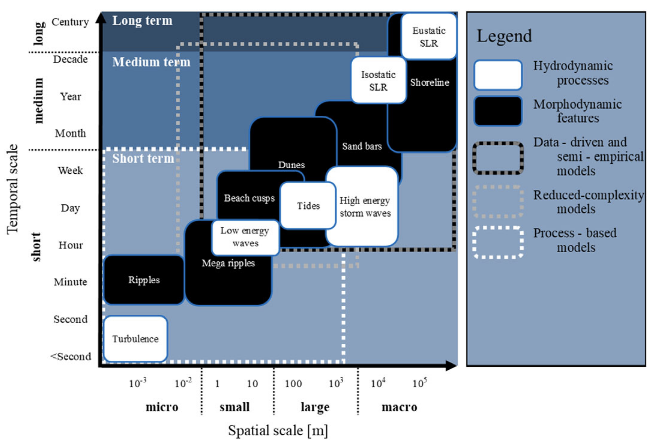
\includegraphics[width=0.8\linewidth]{images/spatial-and-temporal.png}
    \caption{A schematic diagram representing approximate spatial and temporal modelling scales that are appropriate to hydrodynamic processes (white box) and morphodynamic features (black box). Reproduced from Hunt et al. (2023) \textsuperscript{[5]}}
    \label{figure1}
\end{figure}

\par{Erosion and deposition of sediment caused by wave action generated by wind blowing over large stretches of ocean is the predominant morphological effect on most coasts. This effect is most noticeable by observing the of the extent of differences in geographical features between coasts which regularly experience high-wave energy to those which do not.~\textsuperscript{[5]}~\textsuperscript{[6]} As waves propagate from the ocean to the nearshore domain (the subaqueous zone commonly spanning 100m directly seaward of the shoreline) they dissipate as depth decreases to beneath their height, and their energy compounds with that of other hydrological processes occurring at different spatial and time scales such as tides and local currents, to dictate an overall circulatory and sedimentary gradient of the area and in turn influence other ecological, geological, and geographical gradients. By this token, characterizing the hydrodynamics of the coastal zone is essential to understanding all other processes there, and the ability to successfully develop methods for sampling them.~\textsuperscript{[7]}}

\subsection{Hydrological}

\begin{figure} 
    \centering
    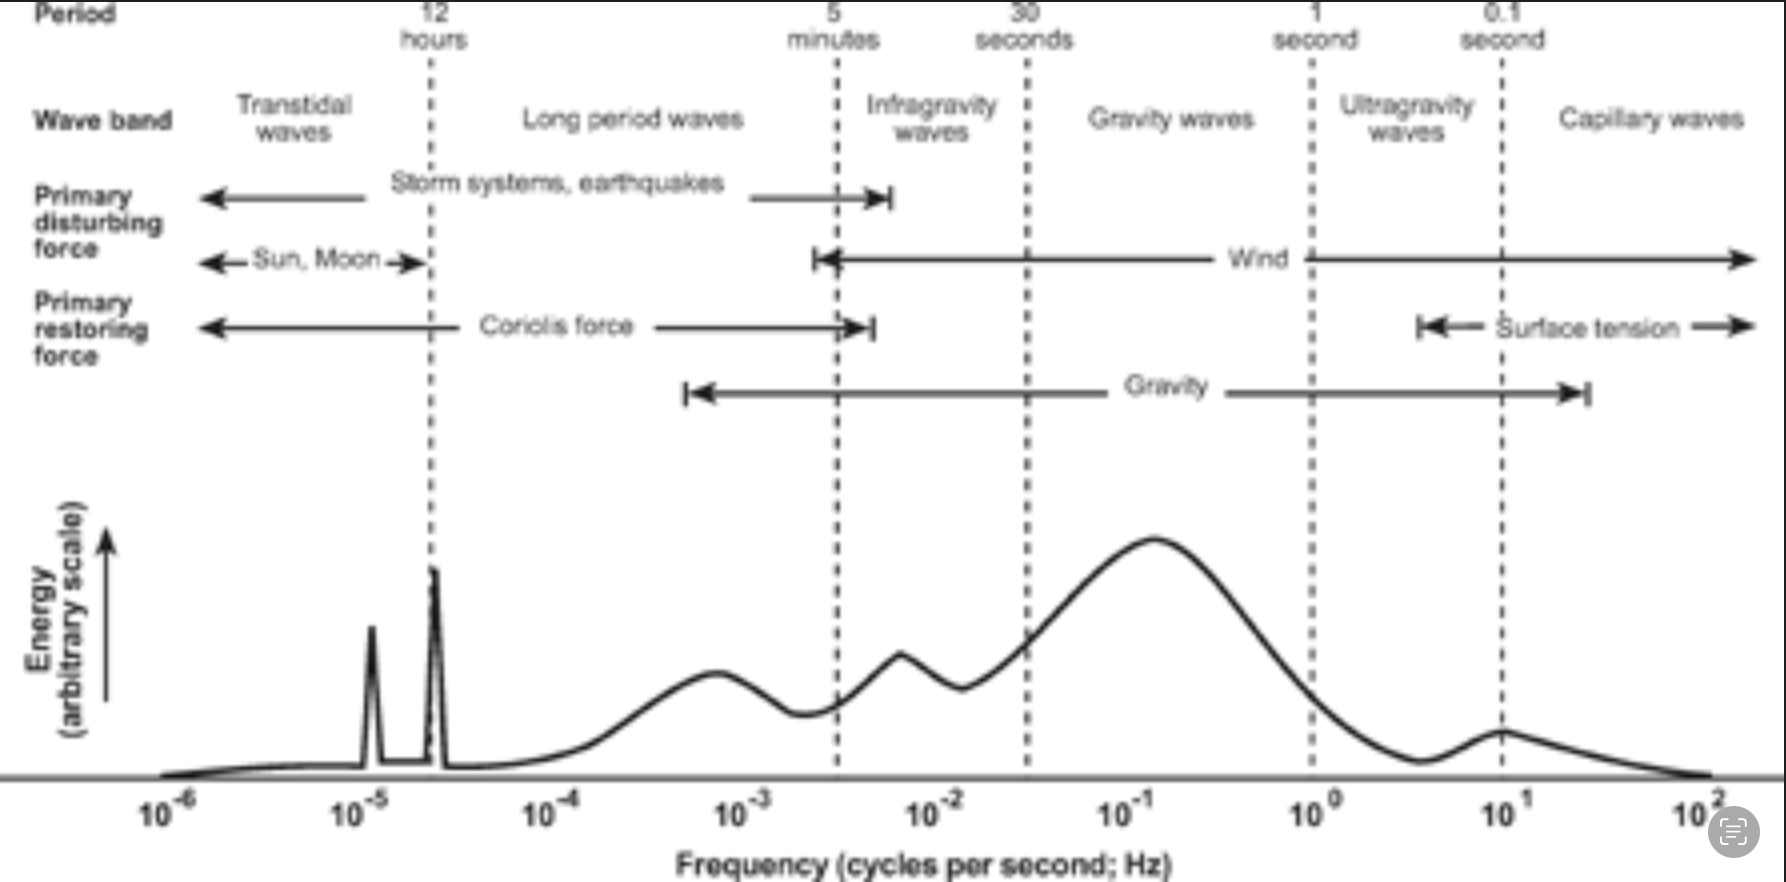
\includegraphics[width=1\linewidth]{images/ocean-wave-energy-schematic.png}
    \caption{Placeholder for self generated graphic based on this one from Kinsman, 1984\textsuperscript{[14]}}
    \label{figure2}
\end{figure}

\par{Ocean waves are created when a disturbing force acts on the ocean and a restoring force acts to restore equilibrium. These forces produce waves of varied frequency, wavelength, height, and direction, which compound to constitute the full spectrum of nearshore hydrodynamic activity. \textsuperscript{[6]}~\textsuperscript{[7]}~\textsuperscript{[11]}~\textsuperscript{[14]} The most commonly observable waves are wind waves: those generated by friction drag from wind blowing over an area of the ocean's surface, transferring energy into the to water.~\textsuperscript{[6]}~\textsuperscript{[7]}~\textsuperscript{[8]}~\textsuperscript{[9]}~\textsuperscript{[14]} A sea is area in which strong winds actively work to generate irregularly peaked waves of varied periodicity traveling in a broad spectrum of direction, resulting in a chaotic ocean surface. When energy losses from waves breaking are offset by energy gained from blowing wind, the sea is said to be fully developed or arisen.~\textsuperscript{[9]}~\textsuperscript{[14]}~\textsuperscript{[15]} The power spectra of a fully developed sea, first proposed by Willard Peirson and Lionel Moskowitz, is well defined, and allows forecasters to accurately model wave conditions based on wind speed and direction.~\cref{figure3}.~\textsuperscript{[11]}~\textsuperscript{[15]}}

\par{To describe the processes by which wind generates waves with more granularity, wind blowing over the ocean stretches the waters surface, and as surface tension works to restore it to equilibrium, capillary (low energy, short wavelength, high frequency) waves, are formed. As wind continues to blow, capillary waves are compounded by wind energy and grow. Capillary waves with a steepness that exceed a wavelength of 1.74 cm become gravity waves. At this threshold, gravity supersedes surface tension as the prevailing restoring force, and works to pull the crest of a wave downward. The water's inertia causes the crests to overshoot and become troughs, inducing a cycle in which water molecules oscillate in a near-frictionless orbit as gravitational forces work to restore the fluid to a state of equilibrium, allowing them to propagate long distances across the ocean's surface.~\textsuperscript{[6]}~\textsuperscript{[9]}~\textsuperscript{[11]} ~\textsuperscript{[14]} As wind activity ceases or waves move away from the area of generation, they are sorted into packets of uniform wavelength and direction. Gravity waves have a period around .1 Hz and represent the most energetic band of the spectra.~\textsuperscript{[6]}~\textsuperscript{[10]}~\textsuperscript{[11]}~\textsuperscript{[15]}.}

\begin{figure}
    \centering
    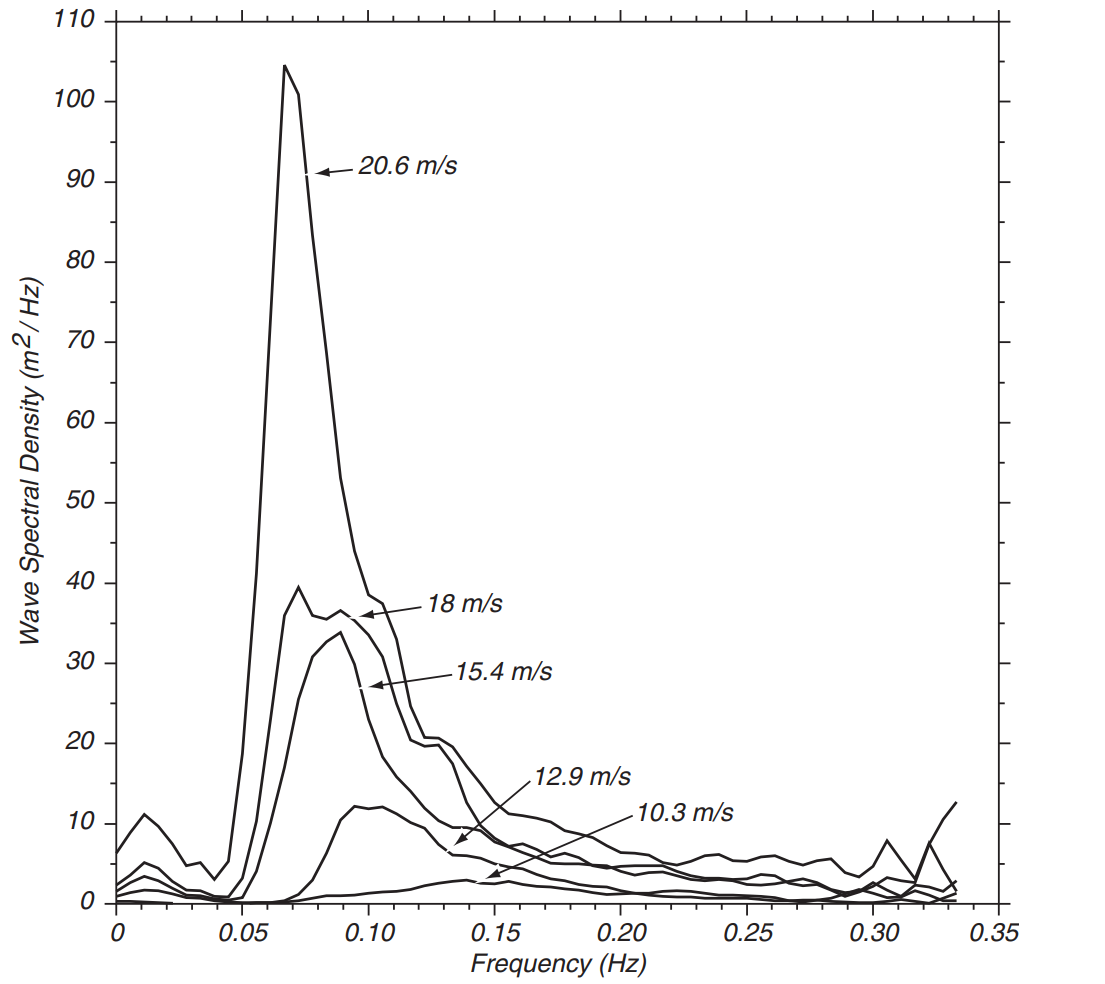
\includegraphics[width=0.75\linewidth]{images/developed-sea-power-spectrum.png}
    \captionof{figure}{Placeholder for self generated version of this Pierson-Moskowitz spectral graph.}
    \label{figure3}
\end{figure}
    
\par{All ocean waves propagate across the surface of the ocean as potential energy, and are released as kinetic energy as they're broken through contact with bottom morphologies and spatial features of the nearshore zone and shoreface.~\textsuperscript{[6]}~\textsuperscript{[7]}~\textsuperscript{[9]} Gravity waves (10-s) compound with phenomenon occurring at longer time scales such as infragravity waves (30 - 300-s), as well as tidal modulation and resulting instabilities from longshore currents (10\textsuperscript{2}-10\textsuperscript{3}-s), to create the full spectrum of nearshore gravity-based wave activity.~\textsuperscript{[7]}~\textsuperscript{[9]}~\textsuperscript{[12]}~\textsuperscript{[13]} Extreme events such as tsunamis generated by seismic activity and seiche (resonant rocking of water) produced by sudden change in atmospheric pressure contribute to nearshore wave activity episodically.~\textsuperscript{[7]}}

\par{The disturbing forces which generate tides are gravitational forces from the moon and sun which act on a rotating earth, causing global variation in local ocean surface height. Isaac Newton, in his work \textit{Principa Mathematica}, postulated the Equilibrium Theory of Tides, which described tides as two bulges of heightened sea level on opposite ends of the earth generated purely as the result of astrological forces acting upon the ocean's surface that remains at a state of equilibrium imposed by them.~\textsuperscript{[7]}~\textsuperscript{[9]}~\textsuperscript{[11]} Newton's theory was intentionally limited: it assumes infinitely deep oceans, not sufficient to explain how tidal wave height would exceed the depth of the ocean when considering the speed of solar and lunar positional change relative the earth.}

\par{Pierre-Simon Laplace expanded upon Newton's Equilibrium Theory of Tides by formulating the Dynamic Theory of Tides, which additionally incorporated phenomenon such as friction, the earth's rotation, the Coriolis effect, and the shape of oceanic basins, to more accurately characterize tidal behavior.~\textsuperscript{[7]}~\textsuperscript{[11]} The Dynamic Theory of Tides describes tidal waves that circulate about amphidromic points, where the tidal range is zero, counterclockwise in the Northern Hemisphere and clockwise in the Southern. Models incorporating these principles have been successful in predicting tides in accordance with observed behaviors.~\textsuperscript{[7]}~\textsuperscript{[11]}  When considered locally at coastal zones, tides are visible through the shoreline fluctuation between low and high tide once (diurnal) or twice (semidiurnal) daily depending on location relative to amphidromic points. These shifts generate longshore currents parallel to all coasts, and cross shore currents where tidal floods and ebbs rush into and out of enclosed areas such as estuaries and other inlets.~\textsuperscript{[7]}~\textsuperscript{[9]} Tidal activity can dominate local sediment transport, and in turn differentiates morphological, geological, and ecological features in some sections of coast, distinguishing them from those with sediment transport dominated by wave action.~\textsuperscript{[11]}}

\begin{figure}
    \centering
    \includegraphics[width=0.75\linewidth]{images/eustatic-sea-level-change.png}
    \caption{Placeholder for self generated version of this graph from Chappell and Shackelton 1986.~\textsuperscript{[18]}}
    \label{figure4}
\end{figure}

\par{The most infrequent hydrodynamic processes which effect coastal waters is eustatic sea level change, or cumulative changes in the volume of the ocean from factors which occur over periods of 10\textsuperscript{5} years or longer, such as addition of water through glacial melting and volcanic out-gassing, thermal expansion of water, and changes in the shape of the seafloor through sediment deposit and tectonic spreading.~\textsuperscript{[4]}~\textsuperscript{[6]}~\textsuperscript{[17]} Local isostatic changes of land level with respect to sea height is caused by tectonic uplift from lithospheric convergence over a period of decades.~\textsuperscript{[6]}~\textsuperscript{[17]} These processes have the most significant influence on shoreline change over longer timescales.~\textsuperscript{[4]} Sea levels have been continuously rising for the past \textasciitilde20,000 years since the Last Glacial Maximum (LGM), primarily caused by the melting of ice sheets from the Last Pleistocene, which has formed today's coastal and inland hydrological features through continental inundation of low-lying areas to form river systems and estuaries and the exposure of fjords previously filled with ice.~\textsuperscript{[6]}~\textsuperscript{[8]}~\textsuperscript{[17]}~\textsuperscript{[18]}~\textsuperscript{[19]}}

\par{Fluvial systems also work to influence coastal processes, in areas where significant amounts of water flows from inland into river deltas and estuaries.~\textsuperscript{[9]}~\textsuperscript{[20]}~\textsuperscript{[21]}~\textsuperscript{[22]} A turbulent jetstream formed by river discharge flowing into a basin from a river dominates the hydrodynamics of a river mouth. The flow structure and velocity of the jetstream are dictated by the geometry of estuarine structure and are highly subject to episodic phenomenon such as storm surges or flooding events.~\textsuperscript{[20]}~\textsuperscript{[21]}~\textsuperscript{[22]} Where present, fluvial processes combine with tidal and wave action to form the overall hydrological gradient of that coastal locale, and may serve as the prevailing factor in some coastal areas which are well-sheltered from highly energetic marine processes.~\textsuperscript{[9]}~\textsuperscript{[20]}~\textsuperscript{[21]}~\textsuperscript{[22]}}

\subsection{Morphological}

\par{\hspace{.5cm}More nebulous than defining the coastal zone's extents are defining the those of it's sub-areas, each subject to different arrays of hydrodynamic processes, which group to form the full cross-shore (a normal vector from shoreline to sea) profile of a coast. Earlier, we adopted a definition of the coast as being an area where sub-decadal oceanic processes influence local morphology through sediment transport. By that token, it's useful to divide the coastal zone into discrete areas based on the amount of sediment transport occurring locally as a result of marine processes.} 

\par{As per our adopted definition, the furthest extent of a coast is the outer boundary where ocean waves break, and the offshore areas exceeding that boundary are unaffected by wave-action induced sediment transport and thus not included.~\textsuperscript{[2]}~\textsuperscript{[6]}~\textsuperscript{[9]}~\textsuperscript{[16]} Adjacent to that and proximal to the shoreline, is the littoral zone, the greater area in which sediment transport occurs both on in the water and on land.~\textsuperscript{[8]}~\textsuperscript{[16]}}
}

\begin{figure}
    \centering
    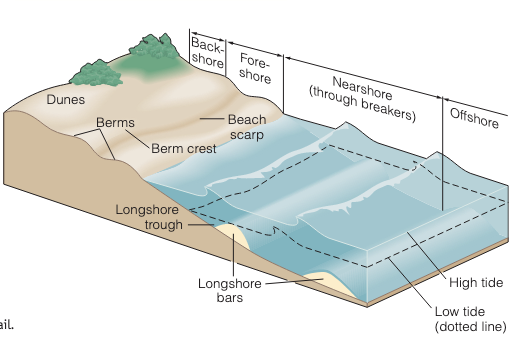
\includegraphics[width=1.0\linewidth]{images/coastal-sub-zones.png}
    \caption{Placeholder for self generated version of this infographic from Essentials of Oceanoraphy~\textsuperscript{[6]}}
    \label{figure5}
\end{figure}

\par{The littoral zone can be divided further into the nearshore, foreshore, and backshore areas~(\cref{figure5}). The seaward limit of the nearshore is the offshore boundary and extends to the shoreline: here waves shoal as depth becomes half the wavelength of incident wave, and break as they come into further contact with bottom morphologies in the surf zone. The foreshore encompasses the area within reach of daily wave and tidal activity, landward from the shoreline and extending to the high-high-water (HHW) mark.~\textsuperscript{[16]} Continuing landward, the backshore area begins at the HHW to the extent of where sediment transport regularly occurs, subject mostly to daily aeolian transport and episodic extreme wave and surge action from storms.~\textsuperscript{[2]}~\textsuperscript{[9]}~\textsuperscript{[12]}~\textsuperscript{[16]}}

\begin{figure}
    \centering
    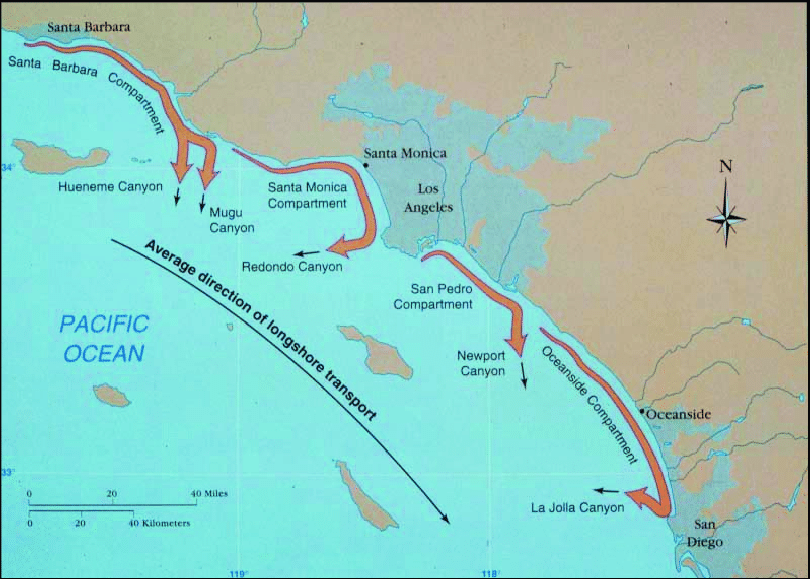
\includegraphics[width=.9\linewidth]{images/so-cal-littoral-cells.png}
    \caption{Placeholder for self generated version of this infographic from Littoral Cells in Southern California by Inman and Chamberlain ~\textsuperscript{[24]}}
    \label{figure6}
\end{figure}

\par{It's also useful to categorize coastlines according to their sedimentary characteristics. One important distinction is between areas of coast which regularly experience a net gain in sediment accumulation as opposed to those which experience a net loss, cateogrized as either depositional and erosional respectively. Another distinction can be made based on the size of sediment grains present onshore, which ranges on a continuum from cliffs and large boulders, to rocks, to sand, to fine-grain mud.~\textsuperscript{[23]} These characteristics manifest into environments which exhibit vastly different morphological, geological, and ecological traits. Sedimentary characteristics are strongly correlated with energy from wave action: often coasts exposed to areas of high wave activity are erosional, as sediment becomes dislodged by wave energy and is transported by longshore currents until it becomes deposited at sheltered beaches nearby.~\textsuperscript{[9]} The geometry of the littoral area also plays a factor: steepness and size of the foreshore and bathymetric gradients in the nearshore correlate to erosional rates and grain size. ~\textsuperscript{[8]}~\textsuperscript{[9]}~\textsuperscript{[16]}~\textsuperscript{[23]}}

\par{Segmenting coastlines according to sediment transport characteristics is also highly pertinent. A coastal or littoral cell is a contiguous sector of coastline in which erosional and accretionary processes are balanced, and spans the distance sediment is transported from an erosional source to the extent to which it is all deposited or lost offshore.~(\cref{figure6}).~\textsuperscript{[9]}~\textsuperscript{[16]} The recognition of discrete littoral cells is essential to understanding and characterizing coastal morphological processes, and is regularly used as a tool in coastal land management and development.~\textsuperscript{[23]} Often littoral cells are bordered by clear geographic markers, such as headlands which restrict the angle of wave approach to the shoreline and disrupt longshore flow, or submarine canyons which channel sediments offshore.~\textsuperscript{[23]}~\textsuperscript{[24]} \par}

\par{Watershed systems are the primary input for sediment into the coastal area, as loose soil particles derived mostly from rain-based erosion are transported downstream to the coast.~\textsuperscript{[8]}~\textsuperscript{[20]}~\textsuperscript{[23]}~\textsuperscript{[25]} In areas subject to high wave activity sediment removed by wave action may exceed sediment deposited from fluvial processes, resulting in erosion.~\textsuperscript{[20]}~\textsuperscript{[26]} Tidal intrusion into estuaries creates currents which interact with jetsteams from fluvial discharge and may create shear fronts and other complex flows which result in unique morphologies.~\textsuperscript{[6]}~\textsuperscript{[8]}~\textsuperscript{[27]} Watershed areas with low wave and tidal activity are more likely to experience sediment accumulation, which may result in depositional landforms such as deltas which penetrate into coastal waters.~\textsuperscript{[6]}~\textsuperscript{[8]}~\textsuperscript{[16]} Anthropic manipulation of watershed systems can also have a significant impact on fluvial sediment transport and deposition, as damming, dredging, and other forms of water management can alter the natural flow of sediment downstream.~\textsuperscript{[16]}~\textsuperscript{[26]}}

\begin{figure}
    \centering
    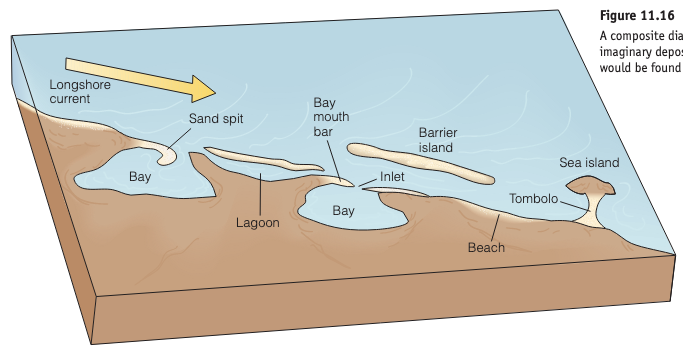
\includegraphics[width=.9\linewidth]{images/coastal-morphology.png}
    \caption{Placeholder for self generated version of this infographic from Essentials of Oceanography ~\textsuperscript{[6]}}
    \label{figure7}
\end{figure}

\par{Many aquatic coastal features were formed as a result of eustatic sea level rise caused by the melting of glaciers since the LGM, which flooded low lying continental areas.~\textsuperscript{[6]}~\textsuperscript{[8]} These features may be categorized according to the influence of different hydrodynamic processes in their formation and composition. Bays are larger bodies of water partially enclosed by land, and can be either fully open to the ocean or partially sheltered by landforms. Lagoons are shallow bodies of salt water that have become partially or fully enclosed by the development of accumulation of sediments into a barrier, or by biological barriers such as reefs, which largely shields them from marine processes.}

\par{Lagoons share crossover with another classifier, estuaries, areas where fresh-water meets and mixes with saltwater. Estuaries are often at the focus of coastal sciences, as they represent some of the most highly dynamic and productive coastal environments. They are generally sheltered from wave action, but may be subject to daily tidal inundation and recession of varying degrees. Estuarine bodies beg further sub-classification, as they can range drastically according their individual hydrological profiles, which in turn dictates how they're formed, as well as the daily fluctuation of their composition. In mountaneous areas of higher latitudes, glaciers formed during the Pleistocene eroded valleys into deep u-shaped troughs, and have since retreaded to create fjords, long narrow marine inlets with steep sides.}

\par{Coastal morphologies in the nearshore and foreshore are formed when sediment is removed or deposited as a result of hydrodynamic processes occuring over time, and so we can categorize morphological features as being either erosional or depositional, each type exhibiting a different array of landform features from one another.}

\par{At erosional coasts, waves break at rock cliffs and disloge debris, which is then transported elsewhere and deposited. Debris can only be disloged at the water line, so cliffs become undercut and develop notches. Notching can cause the cliff above to collapse, or may result in other formations, as weaker zones are removed and others remain to form cliffs such as caves, arches, and stacks. Blowholes can form when erosion continues upwards from a cave to the top of the cliff. The base of notches into a cliffside at the low tide mark which may remain as the cieling above collapses, leaving a large flat wave-cut platform of rock.}

\par{Waves refract in shallow water to break near-parellel to shore, but maintain a slight angle as they crash on the shoreface, resulting in Swash, a turbulent layer of onshore water. Swash rushes up the beach up at the angle of the breaking wave, then retreat straight down towards the shoreline due to gravity, during phases refered to as uprush and backwash respectively. Through uprush and backwash, sediment is loosened and then transported in a zig-zag pattern up and down the beach, with net direction parralel to the coast, in a collective process known as longshore drift. Local properties such as geographic location, shoreline irregularities, nearshore geometry, wind and wave energy, tidal currents, and sediment size, compound to influence how much sediment is removed, how quickly and in which direction sediment is transported, and where it becomes deposited. Sediment will be continuously deposited and transported longshore until the drift is interupted by shoreline irregularitiesx at the end of a littoral cell.}

\begin{figure}
    \centering
    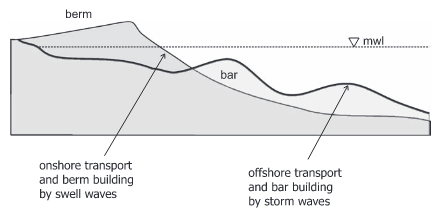
\includegraphics[width=.9\linewidth]{images/barred-profile.png}
    \caption{Placeholder for self generated version of this infographic from Introduction to Coastal Processes and Geomorphology} ~\textsuperscript{[16]}
    \label{figure8}
\end{figure}

\par{Depositional coasts may develop emergent barrier systems of landforms seperated from the mainland by a lagoon, bay, or marsh, which are formed when sediment particles become deposted onto an subaqueous platform or base. }

\par{**Beach topography: Sandy vs rocky, dunes, etc...**}

\par{**Biological effects on morphology: reefs, mangroves, salt flats, etc...**}

\par{**Other factors: volcanism, plate tectonics, glaciers**}

\par{**Geographical effects on erosional / depositional: Trialing edge, roaring 40s, etc...**}

% REFERENCE
\newpage
\fancyhead[C]{REFERENCE}
\fancyfoot[C]{\thepage} 
\thispagestyle{fancy}
\section{Reference}

\begin{enumerate}

    \item {“NOAA’s National Weather Service - Glossary.” Accessed: May 01, 2025. [Online]. \href{https://forecast.weather.gov/glossary.php?word=coastal%20waters}{Available}}
    
    \item {“Definition of the coast,” Geosciences LibreTexts. Accessed: May 01, 2025. [Online]. \href{https://geo.libretexts.org/Bookshelves/Oceanography/Coastal_Dynamics_(Bosboom_and_Stive)/01%3A_Overview/1.05%3A_Coastal_(morpho)_dynamics/1.5.01%3A_Definition_of_the_coast}{Available}}
    
    \item {“Comparative analysis II: Land demarcation and property rights,” in ResearchGate. Accessed: May 04, 2025. [Online]. \href{https://www.researchgate.net/publication/362949604_Comparative_analysis_II_Land_demarcation_and_property_rights}{Available}}
    
    \item {E. Hunt, M. Davidson, E. C. C. Steele, J. D. Amies, T. Scott, and P. Russell, “Shoreline modelling on timescales of days to decades,” Cambridge Prisms: Coastal Futures, vol. 1, p. e16, Jan. 2023, doi: 10.1017/cft.2023.5.}

    \item {M. A. Davidson, K. D. Splinter, and I. L. Turner, “A simple equilibrium model for predicting shoreline change,” Coastal Engineering, vol. 73, pp. 191–202, Mar. 2013, doi: 10.1016/j.coastaleng.2012.11.002.}

    \item {T. Garrison, Essentials of oceanography, 6th ed. Belmont, CA: Brooks/Cole, Cengage Learning, 2012.}

    \item {R. Holman and M. C. Haller, “Remote Sensing of the Nearshore,” Annu. Rev. Mar. Sci., vol. 5, no. 1, pp. 95–113, Jan. 2013, doi: 10.1146/annurev-marine-121211-172408.}

    \item {M. J. Kaiser and P. J. leB Williams, Eds., Marine ecology: processes, systems, and impacts, 2nd ed. Oxford; New York: Oxford University Press, 2011.}

    \item {“Coastal Processes and Beaches | Learn Science at Scitable.” Accessed: May 05, 2025. [Online]. \href{https://www.nature.com/scitable/knowledge/library/coastal-processes-and-beaches-26276621/}{Available}}

    \item {N. US Department of Commerce, “Marine Definitions.” Accessed: May 06, 2025. [Online]. \href{https://www.weather.gov/gum/MarineDefinitions}{Available}}

    \item {G. Masselink, Introduction to coastal processes and geomorphology, Second edition. Oxon [England]: Routledge, 2014. doi: 10.4324/9780203785461.}

    \item {E. B. Thornton and C. S. Kim, “Longshore current and wave height modulation at tidal frequency inside the surf zone,” Journal of Geophysical Research: Oceans, vol. 98, no. C9, pp. 16509–16519, 1993, doi: 10.1029/93JC01440.}

    \item {T. C. Lippmann, A. H. Brookins, and E. B. Thornton, “Wave energy transformation on natural profiles,” Coastal Engineering, vol. 27, no. 1, pp. 1–20, May 1996, doi: 10.1016/0378-3839(95)00036-4.}

    \item {B. Kinsman, Wind Waves: Their Generation and Propagation on the Ocean Surface. New York: Dover Publications, 1984.}

    \item {W. J. Pierson Jr. and L. Moskowitz, “A proposed spectral form for fully developed wind seas based on the similarity theory of S. A. Kitaigorodskii,” Journal of Geophysical Research (1896-1977), vol. 69, no. 24, pp. 5181–5190, 1964, doi: 10.1029/JZ069i024p05181.}

    \item {R. Davidson-Arnott, “An Introduction to Coastal Processes and Geomorphology”.}

    \item {K. Fleming, P. Johnston, D. Zwartz, Y. Yokoyama, K. Lambeck, and J. Chappell, “Refining the eustatic sea-level curve since the Last Glacial Maximum using far- and intermediate-field sites,” Earth and Planetary Science Letters, vol. 163, no. 1, pp. 327–342, Nov. 1998, doi: 10.1016/S0012-821X(98)00198-8.}

    \item {“Coastal prehistory in the southern Red Sea Basin, underwater archaeology, and the Farasan Islands,” ResearchGate. Accessed: May 08, 2025. [Online]. \href{https://www.researchgate.net/publication/277182725_Coastal_prehistory_in_the_southern_Red_Sea_Basin_underwater_archaeology_and_the_Farasan_Islands}{Available}}

    \item {"N. J. Shackleton, “Oxygen isotopes, ice volume and sea level,” Quaternary Science Reviews, vol. 6, no. 3–4, pp. 183–190, Jan. 1987, doi: 10.1016/0277-3791(87)90003-5."}

    \item {"H. Ji, S. Pan, and S. Chen, “Impact of river discharge on hydrodynamics and sedimentary processes at Yellow River Delta,” Marine Geology, vol. 425, p. 106210, Jul. 2020, doi: 10.1016/j.margeo.2020.106210."}

    \item{"C. M. Broaddus et al., “First‐Order River Delta Morphology Is Explained by the Sediment Flux Balance From Rivers, Waves, and Tides,” Geophysical Research Letters, vol. 49, no. 22, p. e2022GL100355, Nov. 2022, doi: 10.1029/2022GL100355."}

    \item{A. Ruiz-Reina, A. López-Ruiz, and M. Ortega-Sánchez, “River Mouth Hydrodynamics: The Role of the Outlet Geometry and Transient Tidal and River Discharge Conditions on the Jet Structure,” Journal of Geophysical Research: Oceans, vol. 130, no. 1, p. e2024JC021500, 2025, doi: 10.1029/2024JC021500.}

    \item{K. Patsch and G. Griggs, “DEVELOPMENT OF SAND BUDGETS FOR CALIFORNIA S MAJOR LITTORAL CELLS”.}

    \item{Littoral cells in Southern California. (Inman and Chamberlain, 1960) Accessed: May 11, 2025. [Online] \href{https://www.researchgate.net/figure/Littoral-cells-in-Southern-California-Inman-and-Chamberlain-1960-Thurman-and_fig4_240635473}{Available}}

    \item{M. M. Alemu, “Integrated Watershed Management and Sedimentation,” Journal of Environmental Protection, vol. 7, no. 4, Art. no. 4, Mar. 2016, doi: 10.4236/jep.2016.74043.}

    \item{A. W. Stevens et al., “Monitoring and modeling dispersal of a submerged nearshore berm at the mouth of the Columbia River, USA,” Coastal Engineering, vol. 181, p. 104285, Apr. 2023, doi: 10.1016/j.coastaleng.2023.104285.}

    \item{W. R. Geyer, D. K. Ralston, M. C. Haller, C. Bassett, and D. Honegger, “The Structure and Dynamics of an Estuarine Tidal Intrusion Front,” Journal of Geophysical Research: Oceans, vol. 129, no. 2, p. e2023JC020371, 2024, doi: 10.1029/2023JC020371.
    }

\end{enumerate}

% END DOCUMENT
\end{document}